\documentclass[en,hazy,black,pc,12pt]{elegantnote}
\usepackage{
amsmath,% AMS basic math stuff
amsthm,% AMS theorem defining stuff
amsfonts,% defines the blackboard bold fonts for \Z, \R, etc
}
%证明符号
\usepackage{bbm}
\usepackage[all,cmtip]{xy}
\usepackage{amssymb}
\renewcommand\qedsymbol{$\blacksquare$}



\newcommand{\rr}{\mathbb{R}}
\newcommand{\msp}{(X,\mathcal{E} ,\mu)}
\newcommand{\psp}{(\Omega ,\mathcal{T}   ,P)}
\newcommand{\cc}{\mathbb{C}}
\newcommand{\cha}{\mathbbm{1}}


\title{Numercial Anaylsis
\\ Based on SU MA232
}

\author{X}
\institute{Elegant\LaTeX{} Program}

\begin{document}

\maketitle

\newpage



%-----------------------------------------------------
\section{Preknowledge}
\subsection{Gaussian elimination and Decomposition de Matrix}

The core of Gussian elimination is 
\[E_nE_{n-1}...E_1 A = U\]

where $E_i$ is the $i$-th elementary row operation and $U$ is the upper triangular matrix.  Above is the langugae of thelinear operator, we can translate each \(E_i\) to be a matrix with a good form to memorilize.

\begin{remark}
    Suppose \(E\) and \(A\) are \(n \times n\) matrix, we call \(E\) an {\bf{elementary matrix}} if it is one of the following three types:
\begin{itemize}
    \item Row addition matrix: \(L_i+aL_j \ra L_i\)
\[E = \begin{bmatrix}
    1 \\
    & \ddots\\
    & a & \ddots\\
    & & & 1 
    \end{bmatrix}, \qquad E_{i,j}=a\]
    \item Row swap matrix: \(L_i \leftrightarrow L_j\)
    \[E= \begin{bmatrix}
        1\\
        & \ddots\\
        & & 0 & & & 1\\
        & & & \ddots\\
        & 1 & & & 0 \\
        & & & & & \ddots\\ 
        & & & & & & 1
    \end{bmatrix}, \qquad 
    \begin{cases}
        E_{i,j}=E_{j,i}=1 \\
        E_{i,i}=E_{j,j}=0 \\
    \end{cases}\]
    \item Row multiplication matrix: \(L_i \ra aL_i\)
    \[E = \begin{bmatrix}
        1\\
        & \ddots\\
        & & a \\
        & & & \ddots \\
        & & & & 1
    \end{bmatrix}, \qquad E_{i,i} = a\]

\end{itemize}

\end{remark}

It is easy to find the inverse of the above matrices, notice that in the case of row addition, if the scalar \(a\) is at \((i,j)\) upon the diagonal, than \(EA\) denotes the column addition \(C_j + aC_i \ra C_j\), ususally we do not need it and we just use row operation, which is more clear and convienient.

\subsection{LU decomposition}
\begin{definition}[Principal Minor]
    For a \(n \times n\) matrix \(A\) we can define its k order principal minor by \[\Delta_k = det\begin{pmatrix}
        a_{11} & a_{12} & \cdots & a_{1k} \\
a_{21} & a_{22} & \cdots & a_{2k} \\
\vdots & \vdots & \ddots & \vdots \\
a_{k1} & a_{k2} & \cdots & a_{kk}
    \end{pmatrix}, \quad k=1,\ldots,n\]
\end{definition}

From Guassian elimination, we can get the \textbf{row echelon form} of a matrix by row operation to get a upper triangular matrix, so for any matrix \(A\) there exists the upper triangular \(U\) such that 
\[ A = E_1^{-1}E_2^{-1}...E_n^{-1}U \]
If row operation does not contain row swap, it is easy to find that the composition of all inverse of the row opreations equals to a lower triangular matrix, that is the LU decomposition.

Formally, The LU decompistion of a square matrix is the product of a lower triangular matrix \(L\) and an uppper triangular matrix \(U\) (triangular matrix have no zero at the digonal by its definition ). For convienience, the digonal of the \(L\) are all 1 and we denote the digonal of \(U\) to be \(u_1, \ldots , u_n\). Next we conculde the existence of the decomposition to be a theorem.

\begin{theorem}[LU decomposition]$\\$
(a) If \(A\) is an invertible matrix, then it has at most one LU decomposition\\
(b) A square matrix has an unique LU decomposition if and only if all principal minors are not null.

\begin{proof}
    We firstly prove (a). Suppose there exists two different LU decompositions for matrix, i.e. \(A=LU,A=L'U'\). so we have \(L(L')^{-1} =U'U^{-1} \). A contradiction occurs since the composition of lower (upper) triangular matrices are a lower (upper) triangular matrix, so the only possiblity is that  \(L(L')^{-1} =U'U^{-1}=I \).

    Now we prove the sufficiency of (b). If A has an LU decomposition, then we write A as the form of a block matrix
    \[A=
    \begin{pmatrix}
        A_1 & A_2 \\
        A_3 & A_4
    \end{pmatrix}
    , L=
    \begin{pmatrix}
        L_1 & 0\\
        B & L_2
    \end{pmatrix}
    , U=
    \begin{pmatrix}
        U_1 & C \\
        0 & U_2
    \end{pmatrix}\]
where \(A_1, L_1, U_1\) are the \(k \times k\) matrices, \(A_4, L_2, U_2\) are the \(n-k \times n-k\) matrices, so clearly k order principal minor is 
\[\Delta_k = detA_1 = L_1U_1\neq 0 \]

Finally we prove the necessary part by induction. If \(A\) is an one order square matrix, then \(A = (a) = (1)(a)\) if \(detA = a \neq 0\). Suppose a \(n-1 \times n-1\) matrix has a LU decomposition for \(n \geq 2\) if all its principal minors are not null, then for a \(n \times n\) matrix \(A\) we can write by block matrix with form 
\[A = \begin{pmatrix}
    A_{n-1} & l \\
    l' & a
\end{pmatrix}
= \begin{pmatrix}
    L_{n-1}U_{n-1} & l \\
    l' & a
\end{pmatrix}
= \begin{pmatrix}
    L_{n-1} & 0 \\
    l'U_{n-1}^{-1} & 1
\end{pmatrix}
\begin{pmatrix}
    U_{n-1} & L_{n-1}^{-1}l \\
    0 & a
\end{pmatrix}\]
where \(a\) is a real number and \(l, l'\) are \(n-1 \times 1\) and \(1 \times n-1\) respectively, so we prove the existence of the decomposition. The uniqueness is immediate from (a) since \(\Delta_n = det A \neq 0\).
\end{proof}

\end{theorem}

And there is an useful technique to check the existence of the decomposition, it depends on the property of continous two order principal minor.  We notice that \(\Delta_k = \prod_{i=0}^k u_k = u_k \Delta_{k-1}\) for \(k \geq 2\) if the matrix has LU decomposition, according to this we have two immediate corollaries.

\begin{corollary}
    for any \(k= 2, \ldots ,n\), if \(\Delta_k \neq 0\) but \(\Delta_{k-1} =0\), then the matrix does not have LU decomposition.
\end{corollary}

\begin{corollary}
    The digonal elements of the upper triangular matrix in LU decomosition is 
    \[ \begin{cases}
        u_k = \Delta_k / \Delta_{k-1} , k \geq 2\\
        u_1 = \Delta_1 
    \end{cases}\]
\end{corollary}



\subsection{Cholesky Decomposition}

LU Descomposition can be finer by add a digonal matrix \(D\), then we can get a LDV decomposition with the following form
\[
LDV=\begin{pmatrix}
    1 & 0      & 0      & \cdots & 0 \\
    l_{21} & 1 & 0      & \cdots & 0 \\
    l_{31} & l_{32} & 1 & \cdots & 0 \\
    \vdots & \vdots & \vdots & \ddots & \vdots \\
    l_{n1} & l_{n2} & l_{n3} & \cdots & 1
\end{pmatrix}
\begin{pmatrix}
    d_1 & 0   & 0   & \cdots & 0 \\
    0   & d_2 & 0   & \cdots & 0 \\
    0   & 0   & d_3 & \cdots & 0 \\
    \vdots & \vdots & \vdots & \ddots & \vdots \\
    0   & 0   & 0   & \cdots & d_n
\end{pmatrix}
\begin{pmatrix}
    1 & u_{12} & u_{13} & \cdots & u_{1n} \\
    0 & 1      & u_{23} & \cdots & u_{2n} \\
    0 & 0      & 1      & \cdots & u_{3n} \\
    \vdots & \vdots & \vdots & \ddots & \vdots \\
    0 & 0      & 0      & \cdots & 1
\end{pmatrix}
\]

If we dsitribute weights in average from digonal matrix to two triangular matrices by \(D=\Sigma^2\), and if the decomposed matrix has a good property , then we can get the decomposition form like \(A = HH^T\), which is the Cholesky decomposition, a more effective technique than LU decompistion.when solving linear equation.

It is not difficult to find that one good property is symmetric since \((HH^T)^T=HH^T\). Positive is an other propery to make the digonal elements in the digonal matrix to be positive. we conculde it by following theorem.

\begin{theorem} A square matrix has a Cholesky decomposition if and only if  it is symmetric and positive-definite.

    \begin{proof}
        We only prove the necessary of the porposition since the sufficiency is easy. we first prove that the principal matrix is all symmetric and positive-definite. Suppose \(A_k = (a_{i,j})_{1 \leq i,j \leq k}\) is the k order principal matrix of \(A\). Clearly, \(A_k\) is symmetric. Since \(A\) is positive-definite, then 
        \[ X^TA_kX = \begin{pmatrix}
            X & 0
        \end{pmatrix}
        \begin{pmatrix}
            A_k & B \\
            C & D
        \end{pmatrix}
        \begin{pmatrix}
            X\\
            0
        \end{pmatrix} > 0\]
        where \(X\) is a k order non-zero vector.

        An symmetric and positive-definite matrix must be invertible, otherwise there existe \(X \in \R^k-\{0\}\) such that \(A^k X = 0\), which implies \(X^TA^kX = 0\). Hence all principal minors are not null, and the matrix has an unique LDV decomposition. Similarly, \(A^T\) also has an unique LDV decomposition, so it implise \(L^T = V\), so if we let \(D = \Sigma^2\), then \(H = L \Sigma\) such that \(A  = HH^T\).
    \end{proof}
\end{theorem}

\section{Numercial \sch for ODE}
\Sch is a vocabulary from french, in nmumercial anaylsis it can be thought as a progam to approximate the real function or an equation. Specially, each numercial method refers to a \textbf{algorithm} of the sequence which converges to the real value, for example, the Eluer method to some Cauchy problem  can be wirte by a recurrance like
\[ y_{n+1} = y_n + hf(t_n, y_n)\]
It implies what the sequence is or what the method of approximation is. We call the recurrance equation contianing all information "\sch ".

In this part, \textbf{Truncation error} is the important concept, it often happens when  replacing infinite precision or infinite process by finite number of calculations. For example, the form of series of exponential functions can be written as 
\[e^x = 1 + x + \frac{e^x}{2!} + \dots\]
If we just choose part of terms to approximate \(e^x\) then error occurs, and Talyor-Lagrange theorem gives the boudary of the errors
\subsection{ExplicIt \sch}
The explicit \sch is the equation with the following equation:
\begin{equation} 
    y_{n+1} = y_n +hF(t_n, y_n,h)
    \label{eq:explicit_scheme}
\end{equation}
where \(F\) is a continuous function defined on \([0,T]\times \R^m \times [0,1]\). 

\begin{definition}[Convergence]$\\$
    The \sch (\ref{eq:explicit_scheme}) is convergent if for any given intial codition \(y(0)\), the continuous problem satisfies
\[
\lim _{\substack{h \rightarrow 0 \\ y_0^N \rightarrow y(0)}} \sup _{0 \leq n \leq N}\left\|y_n^N-y\left(t_n\right)\right\|=0
\]
\end{definition}

\begin{definition}[Stable] $\\$
    Le schéma ~\ref{eq:explicit_scheme} est stable s'il existe une constante \(C\) indépendante de \(N\) telle que, pour toute suite de vecteurs \(\left(\eta_n\right)_{0 \leq n \leq N}\), les suites \(\left(y_n\right)_{0 \leq n \leq N}\) et \(\left(z_n\right)_{0 \leq n \leq N}\) de \(\mathbb{R}^m\) définies respectivement par

\[\begin{cases}
     y_{n+1}=y_n+h F\left(t_n, y_n, h\right) \quad ,0 \leq n \leq N-1 \\ 
    z_{n+1}=z_n+h F\left(t_n, z_n, h\right)+\eta_{n+1} \quad ,0 \leq n \leq N-1 \\
    z_{0} = y_0 +\eta_0
\end{cases}
\]

sont telles que
\[
\max _{0 \leq n \leq N}\left\|z_n-y_n\right\| \leq C \sum_{n=0}^N\left\|\eta_n\right\|
\]
\end{definition}

\begin{remark}
    Let us consider the motivation of the definition. For a discrete numercial method with initial value known, we start the algorithm from \(t_0\), then let \(z_n = y(t_n)\) be the sequence of the real value at \(t_n\), then at \(t_1\) clearly we can deduce that 
    \[\begin{cases}
        y_1 = y_0 + h F(t_0,y_0,h) \\
        z_1 = y_1 + \varepsilon_1 = z_0 + h F(t_0,z_0,h) + \varepsilon_1
    \end{cases}\]
    where \(\varepsilon_1\) is the error between real value and approximation, we call it \textbf{Local Truncation Error (\l'erreur de discrétisation)},but when we repeated algorithm we can get that
    \[z_2 = z_1 + h F(t_1,z_1,h) + \varepsilon_2\]
    where \(\varepsilon_2\) is the LTE between  real value \(y(t_2)\) and apporximation of \(y(t_2)\) starting from real value \(y(t_1)\), and the iteration contains the previous error \(\varepsilon_1\) in it. Hence the difference between \(y(t_2)\) and \(y_2\) relates to the two LTE. We define the\textbf{ Global Truncation Error (\l'erreur de \sch)} with the form
    \[\max _{0 \leq n \leq N}\left\|z_n-y_n\right\|\]
    So the definition of stable \sch means that \textbf{the GTE is bounded by the sum of LTE.}
    \begin{figure}[h]
        \centering
        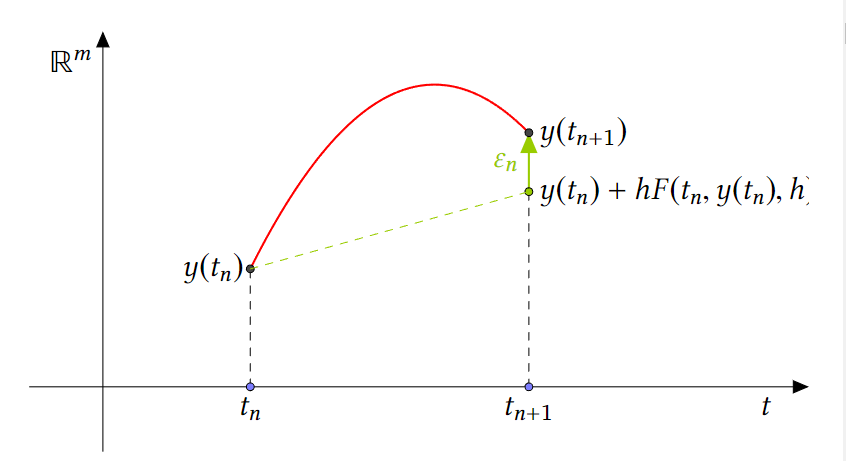
\includegraphics[width=0.8\textwidth]{fig/stable.png}
        \caption{Local Truncation Error}
    \end{figure}
\end{remark}

\begin{definition}[Consistent]
    The sch (\ref{eq:explicit_scheme}) is consistent with the corresponding ODE if for any solution of the ODE \(y(x)\) we have 
    \[
\lim _{h \rightarrow 0} \sum_{n=0}^{N-1}\left\|\varepsilon_n\right\|=0
\]
where \(\varepsilon_n = y(t_{n+1}) - y(t_n)-hF(t_n,y(t_n),h)\) is LTE.
\end{definition} 

Immediately we can get the sufficant condition for the convergence of \sch by the squeezes theorem, where stable property ensures the inequality and consistent property controls the limit.
\begin{theorem}[convergence of explicit \sch]$\\$
    The explicit \sch is convergent if it is stable and consistent.
\end{theorem}

We omit the proof and consider how to determine that a explicit \sch is stable and consistent, we conclude the condition below.

\begin{proposition}
    Consider the \sch (\ref{eq:explicit_scheme})
    \\(a) It is stable if \(F(t,y,z)\) is Lipschitz with respect to variable \(y\)
    \\(b) It is consistent if and only if  \(F(t,y,0) = f(t,y)\) for any \((t,y) \in [0,T] \times \R^m\), where \(f\) is function in the corresponding Cauchy problem.
\end{proposition}

\subsection{Implicit \sch}
The implicit \sch is the equation with the following equation:
\begin{equation} 
    y_{n+1} = y_n +hF(t_n, y_n,y_{n+1},h)
    \label{eq:implicit_scheme}
\end{equation}
where \(F\) is a continuous function defined on \([0,T]\times \R^m \times \R^m \times [0,1]\). 

\begin{remark}
    Suppose \(\phi(Z) = y_n + hF(t_n,y_n,z,h)\), then the recurrance of the sequence is equivalent to the equation \(z = \phi(z)\), so we should verify that the sequence given by \sch is well-defined.

    To make \(\phi\) is a contraction function, we add a condition that \(F(t,y,z,h)\) is L-Lipschitz with respect to \(z\), then we have inequality
    \[ \|\phi(z) - \phi(z)\| \leq |hL| \| z-z'\| \]
    Which means if \(h < 1/L\), then by \textbf{fixed point theorem} the sequence is well-defined.
\end{remark}

Similarly, we can define stable and consistent like what we do in the previous section ( just turn \(F(t_n,y_n,y_{n+1},h)\) into \(F(t_n,y_n,h)\) ), then the Local Truncation Error is
\[\varepsilon_n = y(t_{n+1})-y(t_n)-hF(t_n,y(t_n),y(t_{n+1}),h)\]

We conclude the same result about convergent of the \sch.

\begin{proposition}
    For the implicit \sch (\ref{eq:implicit_scheme})
    \\(a) If \(F(t,y,z,h)\) is L-Lipschitz with respect to variable \(z\) and \(y\), then for any \(h< 1/L\), the \sch is stable
    \\(b) If \(F(t,y,y,h) = f(t,y)\) for any \((t,y) \in [0,T] \times \R^m\), then the \sch is consistent.
\end{proposition}

\begin{theorem} 
    The implicit \sch is convergent if it is stable and consisten.
\end{theorem}

\section{Newton's Method}
 
\subsection{One-dimension method}

We suppose \(y=f(x)\) is a class \(C^1\) real function with a root \(x^\star\), the tangent line at \((x,f(x))\) can be described by
\[ Y = f'(x)(x-x_0) + f(x_0)\]
Let \(Y=0\) we can find the point of intersection of the tangent line at x-axis, the formula is that 
\[x' = x^\star - \frac{f(x^\star)}{f'(x^\star)}\]
Accroding to this, we can define a function \(h_f(x) = x - \frac{f(x)}{f'(x)}\), which maps \(x\) to the intesection of the tangent line at \(x\) with x-axis, so we can give a recurrance for some class \(C^1\) function defined on \([a,b]\) 
\[\begin{cases}
  x_0 \text{ near } x^\star \\
  x_{n+1} = h_f(x_n)
\end{cases}\]
we call it \textbf{Newton sequence}. Then we will consider seveal questions: Is it the sequence well-defined? Does the sequence converge to the root? If it converges, What's the rate of the convergence? We response it by the following theorem:

\begin{theorem}[Quadratic convergence of Newton Method]$\\$
  Suppose that \(f\) is a class \(C^2\) function with a root at \(c\), if \(f\) defined on \(I = [c-r,c+r]\) and \(f'(x) \neq 0\) on \(I\), then there exist postive value \(a, K\) such that Newton sequence 
  \[\begin{cases}
    x_0 \in (c-a, c+a) \\
    x_{n+1} = x_n - \frac{f(x_n)}{f'(x_n)}
  \end{cases}\]
  converges to \(c\) with quadratic estimation
  \[ |x_n - c| \leq \frac{1}{K} (K|x_0 -c|)^{2^n}\]
  where \(K = \frac{\max_{x \in I} |f''(x)|}{2 \min_{x\in I} |f'(x)|}\), \(a = \min (r, 1/K)\).

  \begin{proof}
    \(f'(x)\) is not null dans \(I\) means that iteration will be endless, so we just need to there exist a subinterval such that \(h_f\) is invriant on it, which ensures that the sequence is well-defined. By the formula of Taylor with Reminder,
\begin{align*}
    0 = f(c) &= f(x+(c-x) \\
&= f(x) + (c-x)f'(x)+\frac{(c-x)^2}{2}g''(\eta)
\end{align*}
with \(x\in I\) and \(\eta\) is between \(x\) and \(c\), rearranging it implies 
\[
\left(x-\frac{f(x)}{f^{\prime}(x)}\right)-c=\frac{(c-x)^2}{2} \frac{f^{\prime \prime}(\eta)}{f^{\prime}(x)}
\]
which gives 
\[
|h_f(x)-c| \leq \frac{\max_{x \in I} |f''(x)|}{2 \min_{x\in I} |f'(x)|}|x-c|^2 = K|x-c|^2
\]
To make \(h_f\) invriant, then \(K|x-c|^2 \leq |x-c|\), so the length of the subinterval must be no larger than \(a = \min (r, 1/K)\) to ensure the sequence to converges \(c\). And the quadratic convergence is clearly.
\qed
  \end{proof}

\end{theorem}

\begin{example}[Héon Method]
    Newton method can bu taken use to approximate the \(\sqrt{2}\), we define \(f(x) = x^2 - 2\), then \(\sqrt{2}\) is the root of the equation 
    \(f(x) = 0\), so the recurrance of the sequence is 
    \[x_{n+1} = x_n - \frac{f(x_n)}{f'(x_n)} = \frac{x_n}{2} + \frac{1}{x_n}  \]
    which is a classic problem in anaylsis.
\end{example}

\subsection{N-dimension method}
We can generalize Newton method to \(\R^n\). We consider the affine map \(g(x) = Ax-b\) with \(A \in M_n(\R)\) and \(b \in \R^n\), if \(A\) is invertible, then the equation \(g(x) = 0\) has the unique solution \(A^{-1}b\), but if \(A\)is not invertible and \(b\) is in the column space of the matrix, then the situation will be complex, because the null space is always convex and connected. 

Let us consider the case of \(n = 2\), we take an affine map \(g(x,y)= (x,0)\), it is clear that the set of solutions is y-axis. However, if we want to aprroxiate the root \((0,0)\), and we choose some point near it to be the first term of Newton sequence, then the sequence can not converge to \((0,0)\) if some term \(x_k\) is at the y-axis (\(h_f(x_{k+1}) = 0\)). That is not aviodable since for any small open ball containning \((0,0)\), there exists \((0,y_0)\) of the null space in the open ball, so we need an concept about the isolation of the root.

\begin{definition}
    We call \(c\) is an isolated zero of the function \(f\) defined on \(U\)if for any \(\varepsilon > 0\), there exists no other zero on \(B(c,\varepsilon) \cap U\).
\end{definition}

\begin{proposition}[Sufficant condition of an isolated zero]$\\$
    Suppose \(f: U \subset \R^n \to \R^n \) is a function defined on an open set, and \(x\) is a zero of the function on \(U\). If f is differentiable and \(D_f(x)\) is invertible, then \(x\) is an isolated zero of the function.
    
    \begin{proof}
       It is a weak form of\textbf{ the local inversion theorem}. Considering a function \(h(y) = D_f(x)^{-1}f(y)\), it is also differentiable, and \(D_h(x) = I\), then by definition of the diffentiable function, we have 
       \begin{align*}
        h(y) &= h(x+y-x) \\
        &= h(x) + I(y-x) + o(\|y-x\|) \\
        &= y-x + \varepsilon(y-x)\|y-x\|
       \end{align*}
       where \(\varepsilon\) converges to 0 when \((y-x)\) converges to 0, so there exists a positive \(r\) such that \(\|x-y\| < r \) implies \(\|\varepsilon\|<1/2\). Again by the triangular inequality \(|x+y| \geq ||x|-|y||\), we have 
       \[\|h(y)\| \geq 1/2 \|y-x\| > 0 \] 
       for any \(0<\|x-y\|<r\), by the definite property of the norm we can conclude that \(x\) is an isolated zero.
       \qed
    \end{proof}
\end{proposition}

The exact form of the Newton iteration can be deduced from Talyor Formula of multivariable functions. We suppose that \(f\) is a class \(C^1\) function with an islated root at c, then 
\[0 = g(c) \approx g(x) + D_f (x) (c-x)\]
for some \(x\) approching \(c\), so we can get 
\[ c \approx x - D_f(x)^{-1} f(x) \]
it gives the recurrance of the Newto method on \(\R^n\) 
\[ \begin{cases}
    x_0 \text{ near } c \\
    x_{n+1} = x_n - D_f(x_n)^{-1} f(x_n)
\end{cases} \]

If the new sequence is well-defined? To prove that we need a toplogical property.

\begin{lemma}
    \( GL_n(\R)\) is open in the norme space \(M_n( \R ) \), where the euipped norm is \(\|A\| = \max_{ 1 \leq i,j \leq n} |a_{i,j}|\).
\end{lemma}

The proof of the Lemma can be found in TD 1 of the course of Topologie, according to this we can prove the convergence theorem in n-dimension.

\begin{theorem}[General quadratic convergence of New Mehod]
    If \(f\) is a class \(C^2\) defined on \(U\) with a zero \(x\), if \(D_f(x)\) is invertible, then there exist an open set and a postive value \(K\)  such that for any given initial conition in it, the Newton sequence is well-defined and converges to \(x\) with rate de convergence
    \[\|x_{k+1}-x\| \leq K \|x_k-x\|^2\]
    
    \begin{proof}
        wait...
    \end{proof}
\end{theorem}

\section{}
\end{document}  
